\documentclass[10pt]{article}
\usepackage[%
left=0.984252in,%
right=0.787402in,%
top=0.787402in,%
bottom=0.787402in,%
paperheight=11in,%
paperwidth=8.5in%
]{geometry}%

\usepackage{xeCJK}
\usepackage{blindtext}
\usepackage[T1]{fontenc}
\usepackage{caption}
\usepackage{graphicx}
\usepackage{textcomp}
\usepackage{fancyhdr}

\pagestyle{fancy}
\fancyhf{}
\fancyhead[R]{\thepage}
\usepackage{float}
\usepackage{alltt}

\setCJKmainfont{AozoraMinchoRegular.ttf}
\setCJKsansfont{AozoraMincho-bold.ttf}


\setCJKmainfont{AozoraMinchoRegular.ttf}
\setCJKsansfont{AozoraMincho-bold.ttf}

\usepackage{indentfirst}

\title{ディジタル技術の基礎}
\author{18NC021 \thanks{情報通信基礎実験1}}
\date{カトリ スザン}
\captionsetup[table]{name=表}
\captionsetup[figure]{name=図}

\begin{document}

\begin{titlepage}
	\maketitle
\end{titlepage}

\tableofcontents
\pagebreak

 

\section{使用機器}
この実験で使用した機器を表1に示す。
\begingroup
\setlength{\tabcolsep}{5pt} % Default value: 6pt
\renewcommand{\arraystretch}{1.5} % Default value: 1
% Parts list table
\begin{table}[H]
    \centering
	\caption{使用機器}
	\begin{tabular}{|l|l|l|}
	    \hline
	    使用機器 & 会社名 & 型番等\\[0.5ex]
		\hline\hline
		AD/DA変換実習装置 & IWATSU &ITF-203	 \\ \hline
		直流電源	& LEADER & 818-3\\ \hline
		直流電圧計  &	 & DSP 1-01 (81BA2033)\\ \hline
        オシロスコープ & IWATSU &	SS-7802 \\ \hline
        発信器 (信号発生器) & KENWOOD &	AG-203D \\ \hline
        LPF & ACTIVEFILTER &	DR-04 \\ \hline
        スピーカー &  &	MM-SPL2N2 \\ \hline
	\end{tabular}
\end{table} 
\endgroup

\section{実験1}
\subsection{実験1.1 : AD 変換と量子化誤差 (アナログ入力とディジタル出力の関係)}

\subsubsection{目的}
アナログ電圧を AD 変換するとき、ディジタル値に変換される動作を確認する。入力信号に対する量子化誤差の 変化について考察する。
\subsubsection{使用機材}
$\bullet$ AD/DA 変換実習装置、直流電源、直流電圧計
\subsubsection{方法}

\begin{enumerate}
\item 図1のように直流電源の出力をAD/DA変換実習装置の入力と直流電圧計に接続する。直流電源の電圧をアナログ入力電圧Vinとする。
\item  AD/DA 変換実習装置のスイッチを次のように設定する。
\begin{itemize}
  \item SW1(マイク/AD 入力):AD 入力 
  \item SW3(サンプリングクロック切換):内部 
  \item SW4(8 ビット/4 ビット):4 ビット 
  \item SW5(AD ユニポーラ/バイポーラ):ユニポーラ 
  \item SW6(スピーカ):OFF 
  \item SW7(DA ユニポーラ/バイポーラ):ユニポーラ SW8(メモリ):OFF
\end{itemize}
\item AD/DA 変換自習装置の電源を ON にする。 
\item 直流電源装置の電源を入れ、OUTPUT を ON にし、current ボリュームを調整し最小限の電流値で CV 状態(青LED) にする。
\item AD/DA 変換実習装置の [スタート/ストップ] スイッチを押し、変換動作を開始する。 変換動作中はスイッチ右のLEDが点滅する。スタート状態では、AD/DA変換実習装置の設定を変更することはできない。ストップ状態で変更すること。
\item アナログ入力電圧 Vin を0~3 V まで 0.1V ずつ変化させ、対応した AD 変換器の量子化出力(=ディジタル出力)をメモリ右側 のインジケータの LED${2^7~2^4}$ で観測し、測定データを記録する 。 
\item (a)欄を10進数に変換して(b)欄に記入し、(b)欄の値に量子化単位電圧(0.64V)を乗したVoutを(c)欄に記入する。(d)欄の記入はレポート作成時に行う \\
$\bullet$ 入力電圧に対する AD 変換器の量子化出力と量子化誤差を表 2 に示す。
\item 横軸を Vin、縦軸を Vout として、表2(テキストでは1.1)の結果からグラフを作成せよ。
\end{enumerate}

\subsubsection{回路図}
	\begin{figure}[H]
		\centering
		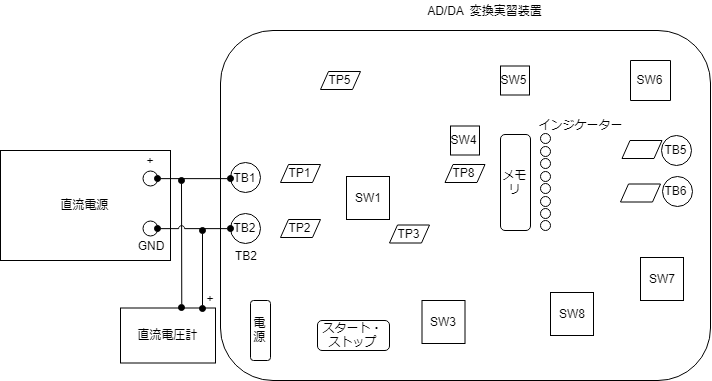
\includegraphics[width=1\textwidth]{exp1.png}
		\caption{実験1回路図}
	\end{figure}
\pagebreak

\subsubsection{実験結果 / 報告事項}

\begin{enumerate}

\item 入力電圧に対する AD 変換器の量子化単位電圧と量子化誤差

\begingroup
\setlength{\tabcolsep}{5pt} % Default value: 6pt
\renewcommand{\arraystretch}{1.5} % Default value: 1
\begin{table}[H]
    \centering
	\caption{入力電圧に対する AD 変換器の量子化単位電圧と量子化誤差}
    \begin{tabular}{|*{5}{c|}}  % repeats {c|} 18 times
    \hline
    \multicolumn{1}{|c}{ } & \multicolumn{3}{|c|}{量子化出力} & \multicolumn{1}{|c|}{} \\ \hline
    \multicolumn{1}{|c}{入力電圧 Vin [V] } & \multicolumn{1}{|c|}{(a)二進数 4bit} & \multicolumn{1}{|c|}{(b) 10進数} &
    \multicolumn{1}{|c|}{(c) 出力値 Vout[V] } & \multicolumn{1}{|c|}{(d) 量子化誤差}\\ \hline
            0.0 & 0000 & 0 & 0.00 & 0.00  \\ \hline
            0.1 & 0000 & 0 & 0.00 & -0.10 \\ \hline
            0.2 & 0000 & 0 & 0.00 & -0.20 \\ \hline
            0.3 & 0000 & 0 & 0.00 & -0.30 \\ \hline
            0.4 & 0000 & 0 & 0.00 & -0.40 \\ \hline
            0.5 & 0000 & 0 & 0.00 & -0.50 \\ \hline
            0.6 & 0001 & 1 & 0.64 & 0.04  \\ \hline
            0.7 & 0001 & 1 & 0.64 & -0.06 \\ \hline
            0.8 & 0001 & 1 & 0.64 & -0.16 \\ \hline
            0.9 & 0001 & 1 & 0.64 & -0.26 \\ \hline
            1.0 & 0001 & 1 & 0.64 & -0.36 \\ \hline
            1.1 & 0001 & 1 & 0.64 & -0.46 \\ \hline
            1.2 & 0010 & 2 & 1.28 & 0.08  \\ \hline
            1.3 & 0010 & 2 & 1.28 & -0.02 \\ \hline
            1.4 & 0010 & 2 & 1.28 & -0.12 \\ \hline
            1.5 & 0010 & 2 & 1.28 & -0.22 \\ \hline
            1.6 & 0010 & 2 & 1.28 & -0.32 \\ \hline
            1.7 & 0010 & 2 & 1.28 & -0.42 \\ \hline
            1.8 & 0011 & 3 & 1.92 & 0.12  \\ \hline
            1.9 & 0011 & 3 & 1.92 & 0.02  \\ \hline
            2.0 & 0011 & 3 & 1.92 & -0.08 \\ \hline
            2.1 & 0011 & 3 & 1.92 & -0.18 \\ \hline
            2.2 & 0011 & 3 & 1.92 & -0.28 \\ \hline
            2.3 & 0011 & 3 & 1.92 & -0.38 \\ \hline
            2.4 & 0011 & 3 & 1.92 & -0.48 \\ \hline
            2.5 & 0011 & 3 & 1.92 & -0.58 \\ \hline
            2.6 & 0100 & 4 & 2.56 & -0.04 \\ \hline
            2.7 & 0100 & 4 & 2.56 & -0.14 \\ \hline
            2.8 & 0100 & 4 & 2.56 & -0.24 \\ \hline
            2.9 & 0100 & 4 & 2.56 & -0.34 \\ \hline
            3.0 & 0100 & 4 & 2.56 & -0.44 \\ \hline
\end{tabular}
\end{table} 
\endgroup
\pagebreak

\item AD変換器の量子化単位電圧と量子化誤差(グラフ)
	\begin{figure}[H]
		\centering
		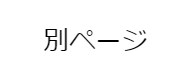
\includegraphics[width=0.2\textwidth]{page.png}
		\caption{AD変換器の入出力電圧(グラフ)}
	\end{figure}
\end{enumerate}
\pagebreak

\subsection{実験1.2 アナログ入力電圧を 4bit で量子化した場合の出力値}
ディジタル出力が変化するときの入力電圧 V(in) を測定する。

\subsubsection{実験方法}

\begin{enumerate}
 \item 接続は図 1 のままで測定する。
 \item アナログ入力電圧 Vin が0 V~10.24V の範囲でインジケータ表示の変化を調べる。
 \item インジケータの表示が次のディジタル値に変化したときの電圧を表 3 にまとめる。
 \item 横軸が入力電圧 Vin、縦軸がディジタル出力の 2 進数として表 3 の結果からグラフを作成する。
\end{enumerate}

\subsubsection{実験結果 / 報告事項}
\begin{enumerate}
    \item 入力電圧に対する AD 変換器の量子化単位電圧と量子化誤差
\end{enumerate}

\begingroup
\setlength{\tabcolsep}{5pt} % Default value: 6pt
\renewcommand{\arraystretch}{1.5} % Default value: 1
% Parts list table
\begin{table}[H]
    \centering
	\caption{AD 変換器のディジタル出力に対応するアナログ入力電圧}
	\begin{tabular}{|l|l|}
		\hline
		ディジタル出力 2進数  & 入力電圧を上昇させ、ディジタル \\  [0.5ex] 
		  &   出力が変化したときのVinの値[V] \\ [0.5ex] 
		\hline\hline
		0000 & 0.00 \\ \hline
        0001 & 0.62 \\ \hline
        0010 & 1.25 \\ \hline
        0011 & 1.89 \\ \hline
        0100 & 2.56 \\ \hline
        0101 & 3.20 \\ \hline
        0110 & 3.80 \\ \hline
        0111 & 4.40 \\ \hline
        1000 & 5.00 \\ \hline
        1001 & 5.70 \\ \hline
        1010 & 6.30 \\ \hline
        1011 & 7.00 \\ \hline
        1100 & 7.60 \\ \hline
        1101 & 8.20 \\ \hline
        1110 & 8.90 \\ \hline
        1111 & 9.60 \\ \hline
	\end{tabular}
\end{table} 
\endgroup

\begin{figure}[H]
		\centering
		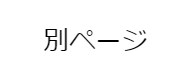
\includegraphics[width=0.2\textwidth]{page.png}
		\caption{AD 変換器のディジタル出力に対応するアナログ入力電圧 (グラフ)}
\end{figure}
\pagebreak

\section{実験3 逐次型AD変換器}
\subsection{目的}
逐次型 AD 変換器を用いて、アナログ電圧をディジタル値に変換する手順を観測し AD 変換器の仕組みを理解する。

\subsubsection{実験方法}
\begin{enumerate}
    \item AD/DA 変換実習装置を以下のように設定する。
        \begin{itemize}
            \item SW1(マイク/AD 入力) :AD 入力 
            \item SW3(サンプリングクロック切換 :内部 
            \item SW4(8 ビット/4 ビット) :8 ビット 
            \item SW5(AD ユニポーラ/バイポーラ):ユニポーラ 
            \item SW6(スピーカー) :OFF 
            \item SW7(DA ユニポーラ/バイポーラ):ユニポーラ 
            \item SW8(メモリ) :OFF
            \item サンプリング周期切換 :5μS
            \item また、オシロスコープのプローブの GND は CH2 を接続し倍率は 10:1 とする。
        \end{itemize}
    \item 直流電源の出力を+7.0Vに設定し変換を開始する
    \item 接続構成を変更しオシロスコープの波形を観測する。\\ この実験の変更前の回路図を図 4、変更後の回路図を図 5 にそれぞれ示す。\\ さらに実験における波形の結果を図 6 に示す。
\end{enumerate}


 
\subsection{回路図}
\subsubsection{AD 変換回路のシーケンス観測接続図(1)}
	\begin{figure}[H]
		\centering
		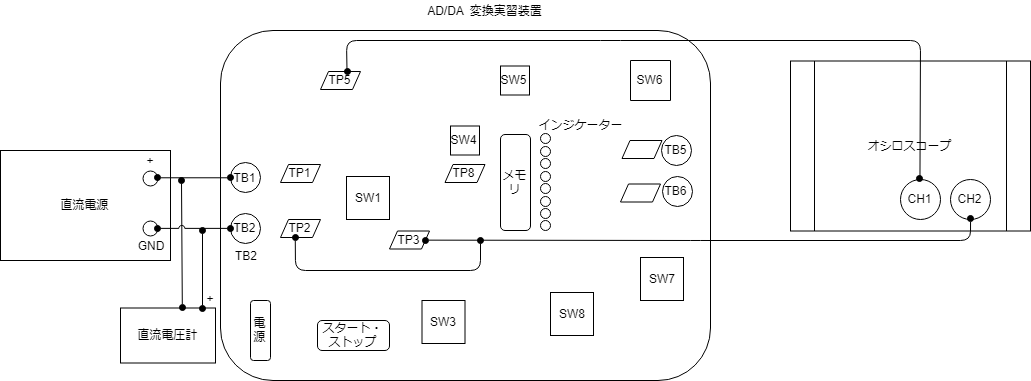
\includegraphics[width=0.8\textwidth]{exp31.png}
		\caption{AD 変換回路のシーケンス観測接続図(1)}
	\end{figure}
	
\subsubsection{AD 変換回路のシーケンス観測接続図(2)}
	\begin{figure}[H]
		\centering
		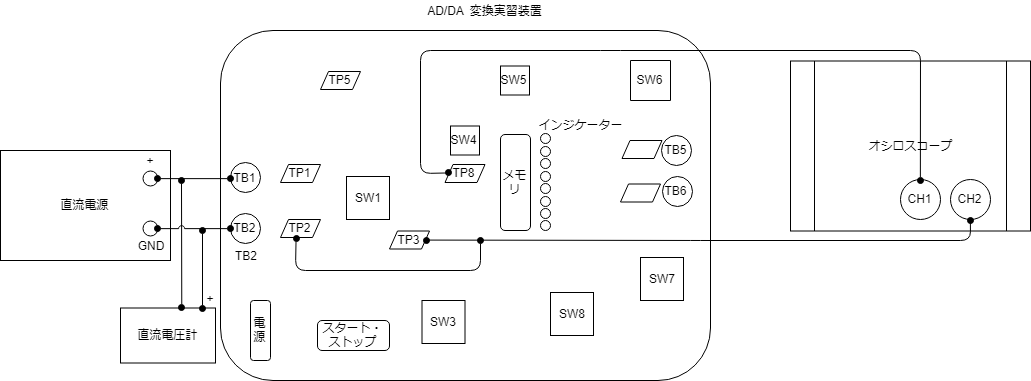
\includegraphics[width=0.8\textwidth]{exp32.png}
		\caption{AD 変換回路のシーケンス観測接続図(2)}
	\end{figure}
 

\subsection{報告事項}
\subsubsection{問題10}

\begingroup
\setlength{\tabcolsep}{5pt} % Default value: 6pt
\renewcommand{\arraystretch}{1.5} % Default value: 1
% Parts list table
\begin{table}[H]
    \centering
    \caption{}
	\begin{tabular}{|llllll|}
	    \hline
	    入力電圧 &  & 電圧単位 ($2^n$ x 0.04) &  & & \\[0.5ex]
		\hline\hline
		7.00v & - & 5.12 (n:7) & = & 1.88 & ... (1)	 \\ \hline
		1.88v & - & 2.56 (n:6) & = & -0.68 & ... (0)	 \\ \hline
		1.88v & - & 1.28 (n:5) & = & 0.60 & ... (1)	 \\ \hline
		0.60v & - & 0.64 (n:4) & = & -0.04 & ... (1)	 \\ \hline
		0.60v & - & 0.32 (n:3) & = & 0.28 & ... (1)	 \\ \hline
		0.28v & - & 0.16 (n:2) & = & 0.12 & ... (1)	 \\ \hline
		0.12v & - & 0.08 (n:1) & = & 0.04 & ... (1)	 \\ \hline
		0.04v & - & 0.04 (n:0) & = & 0.00 & ... (1)	 \\ \hline
		
	\end{tabular}
\end{table} 
\endgroup

\begin{quote}
    \centering
    = $(10101111)^2$
\end{quote}

\begin{quote}
    \centering
    TP8 の信号からディジタル値を読み取り、比較する。 TP8 から読み取れるディジタル値は $(101011110)^2$ で小さい値になった。
\end{quote}



\subsubsection{問題11}
\begin{itemize}
\centering
    \item (b) の対応-0.68[V](1.88-2.56) に相当する。 
    \item TP5 の意味: 入力電圧から 2n ×量子化単位電圧を引いた値 ( TP5 はアナログ値のディジタル的表示を意味し、電圧単位との差を表している。)
    \item TP5 の信号名:DA 変換器の出力
\end{itemize}

\subsection{実験結果}
\begin{figure}[H]
		\centering
		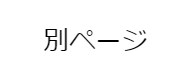
\includegraphics[width=0.2\textwidth]{page.png}
		\caption{波形スケッチ}
\end{figure}

\pagebreak

\section{実験4 人間の手によるAD変換}

\subsubsection{目的}
 波形を人の手でディジタル信号に変換することで AD 変換への理解を深める。 
 
 \subsubsection{実験方法}
 \begin{enumerate}
    \item PC の電源を入れ、MATLAB を起動し、Command Window 画面 (ターミナル)からplay1を実行する。 
    \item Input Digital Data と表示された後、事前にアナログ信号を手でディジタル化して取得した値を入力し、ENTERキーを押す。
    \item 入力したデータに対応した波形が表示されるので配布データと相違がないか確認し問題がなけ ればグラフを閉じる。
    \item "サウンド再生?" とメッセージが表示されるので y、Y を入力し Enter することで入力したディ ジタル信号が DA 変換され音声が再生される。 
    \item 1~4の手順を班員全員のデータが入力されるまで繰り返す。1の Play X は班員の数まで変化さ せる。 
    \item 全員のデータ入力後、Command Window 画面の >>に Playall と入力する。Sound NO と表示 されるので1で作成した play ファイルの数字だけを入力する。 これにより全員分のデータを連続的に再生する。その後全員の音が何かわかるまで再生を続ける。
\end{enumerate}
 音を以下に示す。また事前に AD 変換した自身のデータのトレース結果を図 7 とする。 

\subsection{実験結果 / 報告事項}
\subsubsection{再生音 [あ] (波形プリント1)}
$\bullet$ [3.2,5,6.5,5,3.2,1.6,-0.7,-3.2,-4.2,-3.5,-2.1,-0.1,1.9,1.6,1.6,0.9,0.5,0.9,0.9,1.2,0.7,0,-1.2,-1.9,-2.1,-1.8,\\ -0.3,1,2,1.9,1.1,0.3,-0.4,-0.8,-0.7,-0.2,0,0.1,-0.2,-0.6,-0.6,-0.4,0.2,0.9,1.1,0.9,0.4,-0.3,-0.8,-0.9,-0.7,-0.2,0.2,0.4,\\
0.3,0.1,-0.1,-0.1,0,0.2,0.4,0.3,0.1,-0.1,-0.4,-0.5,-0.4,-0.1,0.2,0.4,0.6];

\begingroup
\setlength{\tabcolsep}{5pt} % Default value: 6pt
\renewcommand{\arraystretch}{1.5} % Default value: 1
% Parts list table
\begin{table}[H]
    \centering
	\caption{実験4 実験結果}
	\begin{tabular}{|l|l|l|}
	    \hline
	      グラフ番号 & play[番号] & 音 \\[0.5ex]
		\hline\hline
		 1 & play2 & あ  \\ \hline
		 2 & play3 & え  \\ \hline
		 3 & play4 & う  \\ \hline
		 4 & play1 & い  \\ \hline
    \end{tabular}
\end{table} 
\endgroup

\begin{figure}[H]
		\centering
		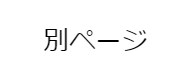
\includegraphics[width=0.2\textwidth]{page.png}
		\caption{(トレース紙) アナログ信号のサンプリング、量子化}
\end{figure}
\pagebreak

\section{実験5  信号発生器入力による折り返し誤差の確認 }

\subsection{目的}
\begin{itemize}
    \item AD 変換器への入力信号がサンプリング定理を満たす場合と満たさない場合の違いを確認する。
\end{itemize}

\subsection{実験方法}

\begin{enumerate}
    \item AD/DA 変換実習装置を以下のように設定する。 
    \begin{itemize}
        \item SW1(マイク/AD 入力)  :AD 入力 
        \item SW3(サンプリングクロック切換 :内部 
        \item SW4(8 ビット/4 ビット)  :8 ビット 
        \item SW5(AD ユニポーラ/バイポーラ) :バイポーラ 
        \item SW6(スピーカー)  :OFF 
        \item SW7(DA ユニポーラ/バイポーラ) :バイポーラ 
        \item SW8(メモリ)   :OFF
        \item また、フィルタはカットオフ周波数 fch=800Hz の端子に接続する。 
    \end{itemize} 
    \item 各装置の電源を起動し信号発生器の周波数は 200Hz 波形をサイン波とし、AD/DA 変換実習 装置のサンプリング周期 T を 500$\mu$s にする。 
    \item スタート/ストップ スイッチから変換を開始し、オシロスコープ画面から CH1 に信号発生 器からの入力信号、CH2 に DA 変換しフィルタを通した出力信号が表示されていることを 確認する。
    \item 信号発生器の出力にコネクタを使い、外部スピーカーを接続する。信号発生器の周波数fを 200~2000Hz の範囲で連続的に変化させ、聞こえる音を確認する
    \item 外部スピーカーとオシロスコープのCH2 をフィルタの出力にコネクタを用いて同時接続する。
    \item 信号発生器の周波数fを 200~2000Hz の範囲で連続的に変化させていき、聞こえる音を4. と比較する。 
    \item オシロスコープで波形を観察する。5. の手順から音を聞きながら波形が観察できる。 信号発生器の周波数fを 200~2000Hz の範囲で連続的に変化させていき CH1(入力)の信 号と CH2(出力)の波形をオシロスコープ画面で比較する。 
    \item 入力信号が 500Hz と 1.5KHz の時の入出力波形をスケッチして比較する。
\end{enumerate}

\subsection{回路図}

\begin{itemize}
    \item この実験における接続図を図 8 に示す。 
\end{itemize}

\begin{figure}[H]
		\centering
		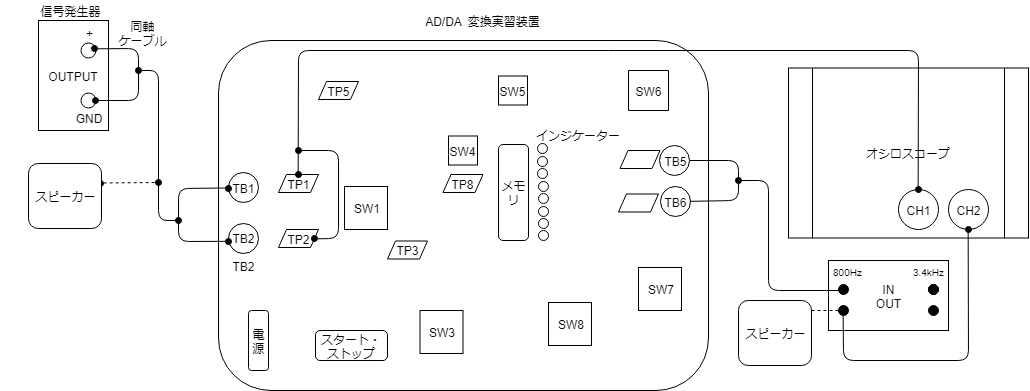
\includegraphics[width=0.8\textwidth]{exp5.png}
		\caption{実験5 接続図}
	\end{figure}

\subsection{実験結果 / 検討事項}

\begin{itemize}
    \item この実験の結果から出力信号の周波数 fout と入力信号 fin との間に成り立つ関係式を表 5 に示し、 測定結果を表 6 に示す。また表 6 から出力周波数のグラフを作成し図 9 に示す。また、8. の結果の スケッチを図 10 とする
\end{itemize}

\subsubsection{信号発生器から入力信号と AD/DA 変換器の出力信号の比較と関係式 }

\begingroup
\setlength{\tabcolsep}{5pt} % Default value: 6pt
\renewcommand{\arraystretch}{1.5} % Default value: 1
% Parts list table
\begin{table}[H]
    \centering
	\caption{信号発生器から入力信号と AD/DA 変換器の出力信号の比較と関係式}
	\begin{tabular}{|l|l|l|l|}
	    \hline
	     & 入力信号 & 出力信号 & 関係式 \\[0.5ex]
		\hline\hline
		 1000Hz以下 & 上昇 & 上昇 & fout = fin \\ \hline
		 1000Hz以上 & 上昇 & 減少 & fout = fs $-$ fin \\ \hline
	\end{tabular}
\end{table} 
\endgroup

\subsubsection{AD/DA 変換器への入力信号に対する出力信号の周波数}

\begingroup
\setlength{\tabcolsep}{5pt} % Default value: 6pt
\renewcommand{\arraystretch}{1.5} % Default value: 1
\begin{table}[H]
    \centering
	\caption{AD/DA 変換器への入力信号に対する出力信号の周波数(サンプリング周期 500μs) }
	\begin{tabular}{|l|l|}
	    \hline
	      入力信号 (CH2) [Hz] & 出力信号 (CH2) [hz]\\[0.5ex]
		\hline\hline
            200  & 200  \\ \hline
            400  & 400  \\ \hline
            600  & 600  \\ \hline
            800  & 800  \\ \hline
            1000 & 1000 \\ \hline
            1200 & 800  \\ \hline
            1400 & 600  \\ \hline
            1600 & 400  \\ \hline
            1800 & 200  \\ \hline
            2000 & 0    \\ \hline
	\end{tabular}
\end{table} 
\endgroup

\subsubsection{グラフ}

\begin{figure}[H]
		\centering
		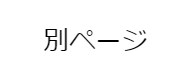
\includegraphics[width=0.2\textwidth]{page.png}
		\caption{実験5 : 入力信号が500Hzの時の入出力波形}
\end{figure}

\begin{figure}[H]
		\centering
		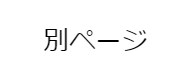
\includegraphics[width=0.2\textwidth]{page.png}
		\caption{実験5 : 入力信号が1.5kHzの時の入出力波形}
\end{figure}
\pagebreak

\section{検討事項}

\subsection{検討事項1}

\begin{itemize}
    \item サンプリングとは何かについて説明せよ。またサンプリング定理について具体的に説 明せよ
\end{itemize}

サンプリング音や映像をデジタルデータに変換する処理のひとつで、一定の間隔でデータを分割して、アナログからデジタルに変換すること。サンプリングは連続信号を一定の間隔をおいて測定することにより、離散信号として収集する。
また、サンプリング定理(標本化定理)とは、アナログ信号をデジタル信号に変換する時、元の信号に含まれる周波数成分の2倍より高い周波数でサンプリングすれば、 元信号を再現することが出来るというものである。例としては最大 500Hz の周波数成分を 標本化したいならば 1000Hz 以上の周波数で標本化する必要がある。 

\subsection{検討事項2}

\begin{itemize}
    \item 量子化とは何かについて説明せよ
\end{itemize}

情報理論や信号処理において、標本化で得られた離散時間信号のようなアナログデータ(連続量)をデジタルデータなどの離散的な値で近似的に表すこと。値をあらわすのに用いるビット数を量子化ビット数と言い、一般に、これを増やして、離散値としてとりうる値の範囲を広げると、量子化誤差が減り、量子化の精度が上がる。 

\subsection{検討事項3}

\begin{itemize}
    \item 実験1の表1.1において量子化誤差Vout-Vin[V]を計算し入力電圧Vin に対する量子化誤差の変 化をグラフにせよ 但し、入力電圧を独立変数(横軸)、量子化誤差を従属変数(縦軸)とせよ。 
\end{itemize}

量子化誤差 Vout-Vin[V]は表 1 に記載 グラフについては図 11 に示す。

\begin{figure}[H]
		\centering
		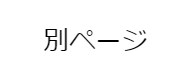
\includegraphics[width=0.2\textwidth]{page.png}
		\caption{入力電圧に対する量子化誤差の変化を表しているグラフ}
\end{figure}
\pagebreak

\subsection{検討事項4}

\begin{itemize}
    \item  3 で得られたグラフについて量子化誤差の変化について考察せよ 
\end{itemize}

実験 1-図 2 のグラフと比較したことにより量子化出力による 2 進数表示の変化に従属しているものと理解できた。また、量子化誤差は一定の 間隔で徐々に大きくなっていくこと、次の値に移行したとき誤差はまた小さくなる 事が理解できた。 

\subsection{検討事項5}

\begin{itemize}
    \item 実験1において A/D 変換器への入力電圧の範囲が 0 ~ 10.24[V]であり、かつ量子化ビット数が 8 ビットである場合の量子化単位電圧を導出せよ 
\end{itemize}

 \begin{quote}
    \centering
    Vmax / $2^{r-1}$ より、\\
 \end{quote}

\begin{quote}
    \centering
    10.24 / $2^{8-1}$ = 0.04[V] \\
 \end{quote}

 
\subsection{検討事項6}
\begin{itemize}
    \item 実験2は行っていない
\end{itemize}

\subsection{検討事項7}

\begin{itemize}
    \item 実験 3 においてサンプル&ホールド回路について具体的に説明せよ 
\end{itemize}
    サンプルモード、ホールドモードの 2 つの動作を行う。             常に変化する信号のある一定の段階で外からのトリガーに合わせて保存するという機能を持つ。
    電圧を大きい順に比較し正ならば1を、負ならば0を当てはめていく。 

 \subsection{検討事項8}
 \begin{itemize}
     \item 実験 3 において入力電圧が 4.30[V]であった場合の A/D 変換の手順を説明せよ。量子化誤差が生 じる場合量子化誤差を示せ。 
 \end{itemize}
 \begingroup
\setlength{\tabcolsep}{5pt} % Default value: 6pt
\renewcommand{\arraystretch}{1.5} % Default value: 1
% Parts list table
\begin{table}[H]
    \centering
    \caption{検討事項8 回答}
	\begin{tabular}{|llllll|}
	    \hline
	    入力電圧 &  & 電圧単位 ($2^n$ x 0.04) &  & & \\[0.5ex]
		\hline\hline
		4.30v & - & 5.12 (n:7) & = & -0.82 & ... (0)	 \\ \hline
		4.30v & - & 2.56 (n:6) & = & 1.74 & ... (1)	 \\ \hline
		1.74v & - & 1.28 (n:5) & = & 0.46 & ... (1)	 \\ \hline
		0.46v & - & 0.64 (n:4) & = & -0.18 & ... (0)	 \\ \hline
		0.46v & - & 0.32 (n:3) & = & 0.14 & ... (1)	 \\ \hline
		0.14v & - & 0.16 (n:2) & = & -0.02 & ... (0)	 \\ \hline
		0.14v & - & 0.08 (n:1) & = & 0.06 & ... (1)	 \\ \hline
		0.06v & - & 0.04 (n:0) & = & 0.02 & ... (1)	 \\ \hline
		
	\end{tabular}
\end{table} 
\endgroup

\begin{quote}
    \centering
    よって01100100量子化誤差0.02[V]
\end{quote}

\subsection{検討事項9}
\begin{itemize}
    \item 実験 5 においてサンプリング定理を満足する入力信号の周波数条件を理由を含めて説明せよ。 
\end{itemize}
\large
実験5の入力信号の最大周波数が2000kHzであるため、標本化定理より 4000kHz 以上 の周波数で行うことが条件となる。

\subsection{検討事項10}
\begin{itemize}
    \item  実験 5 において D/A 変換器の出力にフィルタを接続する理由について説明せよ。 
\end{itemize}
\large
実験1-2よりアナログからディジタルへと変換された場合にデータが階段状に変化することがわかる。、この事からサンプリング周波数の 1/2 を超える周波数成分を含んでいることが分かる。またそのため不要な周波数成分が出力にまじる可能性がある。これらのノイズ要因となりえるものを取り除くため出力に混じっているサンプリング周波数より高い成分を除去する。それ らの為にフィルタが必要である

\section{考察}
\large
今回の実験を通じてアナログ信号をディジタル信号に変換するための基礎的な知識として標本化、サンプリング定理、量子化、量子化誤差、量子化単位電圧の求め方などのについて理解した。実験3の上皿天秤の例ではアナログ信号がどのようにディジタル信号に変換されているかを学習し、人間の手によるAD変換と合わせて自分自身の計算などをしAD変換を行うことでディジタル信号における1が正の数値で0となるものが負の数の値となることを具
体的に理解することができた。

実験4では実際に標本化を行いそれを音声として再生したことからディジタル値というものは離散的なデータであるとこを確認することができた。また、MATLABで波形をプロットし、波を音に変換することで音の波形が実際にどのようなものかを観測することができ、波の性質などについて詳しく理解できた。そしてMATLABの基本的な使い方も学習できた。

信号発生器入力による折り返し誤差の確認実験ではAD/DA変換器の入力信号と
出力信号の関係式の特性を理解することができ、さらに入出力の周波数を観測し
そこから入力信号と出力信号の関係式の特性が成立していることを確認できた。
そして各実験の結果のグラフ、表を書くことにあたってそれぞれの特性の比較や確認の補助
へと繋がり、実験1のように量子化出力のグラフと量子化誤差のグラフの関連性な
どの理解が深まった。

実験2、3、5ではオシロスコープを使って二つ以上の波を観測することで、CRTオシロスコープから値を読み取る方法やCH1とCH2の波を同時に表示させる方法などのオシロスコープの基本的な操作方法についても理解した。

これからは、本実験で学んだことを活かし、実際にフーリエ変換がアナログ信号をディジタルに変換するとき、どのように使われているかについて詳しく学習したい。また、フーリエ変換を使ったオーディオファイルの圧縮などについても詳しく学習したいと思う。

\section{参考文献}

\begin{itemize}
    \item https://ja.wikipedia.org/wiki/アナログ-デジタル変換回路
    \item https://ja.wikipedia.org/wiki/変調方式
    \item http://memes.sakura.ne.jp/memes/?page\_id=1120
    \item https://www.amazon.com/Essential-Guide-Digital-Signal-Processing/dp/0133804429/ref\\=sr\_1\_2?keywords=analog+signal+book&qid=1559393356&s=gateway&sr=8-2
\end{itemize}



\end{document}